\documentclass[12 pct]{report}
\usepackage[utf8]{inputenc}
\usepackage{graphicx}
\usepackage[english]{babel}
\usepackage[left=1.5in, right=1.5in, top=1in, bottom=1in]{geometry}
\graphicspath{ {D:/licenta/soundsPaper/images/} }
\setcounter{section}{-1}

\begin{document}

\title{%
  High frequency audio steganography \\
  \large Practical application \\
    and comparissons with other techniques}

\author{Teodor Paius, coord. Septimiu Crivei}

\maketitle

\begin{abstract}
Steganography is the practice of concealing a file, message, image, or video within another file, message, image, or video. This paper will focus on the domain of digital signal processing and audio concealment of messages. Apart from other common environments such as images or plain text, sound also represents a good way of transmiting hidden messages. The techniques present in this thesis can be applied not only to the target range of human hearing but can also be implemented with some degree of resemblance to other domains of higher frequencies (radio waves or elctro-magnetic waves).
\end{abstract}

\tableofcontents




\chapter{Theoretical background}

The commonly stated range of human hearing is 20 Hz to 20 kHz. Under ideal laboratory conditions, humans can hear sound as low as 12 Hz and as high as 28 kHz, though the threshold increases sharply at 15 kHz in adults, corresponding to the last auditory channel of the cochlea. Humans are most sensitive to (i.e. able to discern at lowest intensity) frequencies between 2,000 and 5,000 Hz. Based on this a good way of hiding information is exploiting this human weakness and encoding certain messages in audio files disguised as short sequences of high frequency signals.




\section{Overview of steganography}
Steganography is the practice of concealing a file, message, image, or video within another file, message, image, or video.
The advantage of steganography over cryptography alone is that the intended secret message does not attract attention to itself as an object of scrutiny. Plainly visible encrypted messages, no matter how unbreakable they are, arouse interest and may in themselves be incriminating in countries in which encryption is illegal.\cite{note4}


\section{Overview of digital signal processing}
To be able to analyze an analog(continous) signal in a digital environment, it must firstly be converted using and analog-to-digital converter. This process is composed of 2 major stages: discretization and quantization. This would transform a continous signal in a set of consecutive frames equidistant in time, and characterized by a certain amplitude.\ref{fig:samp_rate}


\begin{figure}[h]
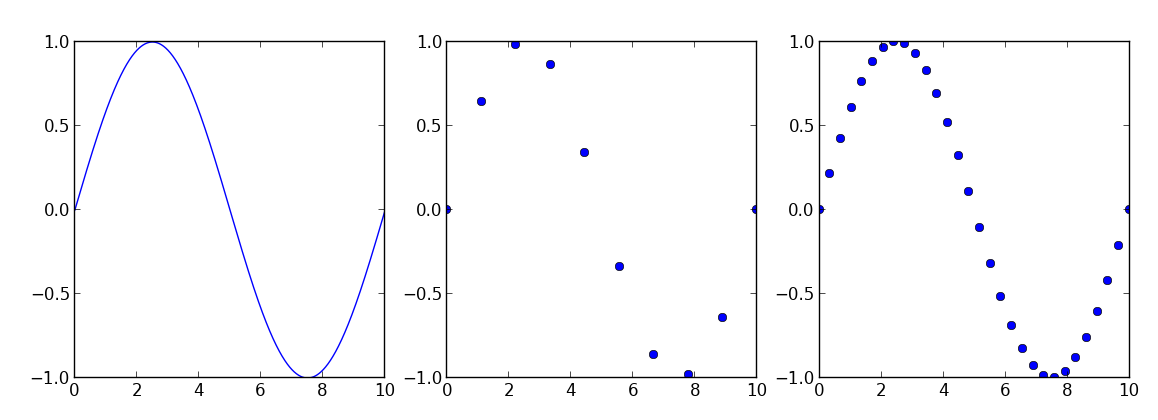
\includegraphics[width=1\textwidth]{sampling_rate}
\centering
\label{fig:samp_rate}
\caption{Continous signal splitted in discrete samples}
\end{figure}

The \emph{Nyquist–Shannon} sampling theorem states that a signal can be exactly reconstructed from its samples if the sampling frequency is greater than twice the highest frequency component in the signal. In practice, the sampling frequency is often significantly higher than twice the Nyquist frequency\cite{note5}. In this case, where the target range is about 20-26 khz, a sampling  rate of 48000 samples/second is almost at the limit, meaning that some higher frequencies might be omitted and loss of accuracy, so a higher sampling rate was chosen: 96000 samples/second.


\section{Just a little bit of anatomy}

\chapter{The application}
For proving the concept of hiding information using high frequency signals, an python application was implemented
\section{Chosen method}


\section{Limitations}
\subsection{Hardware limitations}
\subsection{Software limitations}

\section{Further improvements}

\chapter{Comparison with existent methods}
\section{Other techniques}
\subsection{LSB \emph{(least significant byte}) method}
\subsection{Phase coding}
\section{Advantages/disadvantages}



\begin{thebibliography}{3}
\bibitem{note1}
Katzenbeisser, S., Petitcolas, F.A.P.: Information Hiding: Techniques for steganography 
and digital watermarking. Artech House, Boston (1999) 
\bibitem{note2}
Mahendra Kumar Pandey, Girish Parmar, and Sanjay Patsariya:An Effective Way to Hide the Secret Audio File Using 
High Frequency Manipulation (2011)
\bibitem{note3}
Ahmed Hussain Ali,Mohd Rosmadi Mokhtar and LoayEdwar George: A Review on Audio Steganography Techniques (2015)
\bibitem{note4}
Pahati, OJ (2001-11-29). "Confounding Carnivore: How to Protect Your Online Privacy". AlterNet. Archived from the original on 2007-07-16. Retrieved 2008-09-02.
\bibitem{note5}
Candes, E. J., Wakin, M. B. (2008). An Introduction To Compressive Sampling. IEEE Signal Processing Magazine, 25(2), 21-30. doi:10.1109/MSP.2007.914731
\end{thebibliography}


\end{document}